\documentclass[12pt]{article}
\usepackage{array}
\usepackage{amsmath}
\usepackage{amssymb}
\usepackage{xfrac}
\usepackage{ntheorem}
\usepackage{algorithm}
\usepackage{algorithmic}
\usepackage{caption}
\usepackage{fontspec}
\usepackage{graphicx}
\usepackage{indentfirst}
\usepackage{enumitem}
\usepackage{minted}
\usepackage{mathtools}
\usepackage{pifont}
\usepackage{setspace}
\usepackage{subfigure}
\usepackage{tikz}
\usepackage{url}
\usepackage{tcolorbox}
\usepackage{xcolor}
\usepackage{xeCJK}

\usepackage[colorlinks=true]{hyperref}
\usepackage[margin=0.55in]{geometry}

% background color for minted
\definecolor{bg}{rgb}{0.95,0.95,0.95}

% CJK font
\setCJKmainfont{Source Han Serif CN}

% indent value
\setlength{\parindent}{2em}

% line spacing
\linespread{1.2}
\renewcommand{\thesection}{\Roman{section}}
\renewcommand{\thesubsection}{\thesection-\arabic{subsection}}

\title{An Introduction to the $\lambda$-Calculus}
\author{Yiteng Zhang}

\begin{document}
\maketitle

\noindent{}\textbf{注:}$\lambda$-演算在编程语言理论中有很重要的地位,因而了解与领会其精神还是挺有意义的一件事。
作为了解$\lambda$-演算的材料,这篇文章的内容主要摘自Matthias Felleisen与Matthew Flatt在Utah CS7520中的讲义
\textit{Programming Languages and Lambda Calculi}里有关$\lambda$-演算的介绍部分。

\vspace{1em}
\indent{}\textbf{$\boldsymbol{\lambda}$-演算}是丘奇(Church)提出的,时间略早于图灵(Turing)提出图灵机。
虽然$\lambda$-演算的形式非常简单,但它是图灵完备的,因而它是可以用于模拟任何图灵机的通用模型。
本文的目的是简单地介绍作为语言的$\lambda$-演算,它实际上与一些实用语言(比如Scheme和ML)非常接近。
在这些语言中,函数不仅是用来操作布尔数、整数和序对(pair)的,它们也可以操作其它函数。换言之,函数是值。
举例来说,我们熟知的\texttt{map}函数取一个函数与一个列表(list),并将函数应用到列表的每个元素上。类似地,一个
叫\texttt{derivative}的函数可能会取一个(定义在实数上的)函数,并返回一个实现了该函数导数的新函数。
在$\lambda$-演算中,虽然值的类型只有函数,但我们会看到,其它类型的值(包括布尔数、整数和序对)是可以
用函数来定义的。

\section{$\boldsymbol{\lambda}$-演算中的函数}
\indent{}$\lambda$-演算的句法(syntax)提供了一个简单而规则的书写函数的方法,而函数也可以是其它函数的输入或输出。
在$\lambda$-演算中,这种函数的规范集中于从参数到结果的规则上,并忽略了函数及其域和范围的命名问题。比如,数学上对于
定义在某个集合$A$上的恒等函数的表达是:$\forall x \in A,f(x) = x$,而在$\lambda$-演算中,我们简单地写出
$(\lambda x.x)$这一表达式。它的一种不太正式的读法是:如果参数叫$x$,那么函数的输出也是$x$。
换言之,函数的输出即其输入。

\indent{}对于将一个函数$f$应用到一个参数$a$上的写法,$\lambda$-演算使用了常规的数学表达形式,但使用
成组的小括号将其包在一起:$(f\;a)$。举个例子,将恒等函数应用到参数$a$上的表达式是:$((\lambda x.x)\;a)$。
由于函数也可以是参数,所以将恒等函数应用到恒等函数的表达式是:$((\lambda x.x)\;(\lambda x.x))$。对于
忽略参数并返回恒等函数的函数,我们可以将其表达为:$(\lambda y.(\lambda x.x))$。我们还能写出一些含义更复杂
的函数,比如这样一个函数,其返回是将其参数$x$忽略但返回原函数的参数$y$的函数:$(\lambda y.(\lambda x.y))$。
$\lambda$-演算仅支持单参数函数,但是我们刚才的例子表明一个函数可以有效地取到两个参数$x$与$y$:通过消耗掉
第一个参数$y$接着返回另一个函数来拿到第二个参数$x$。这种技术被称为\textbf{柯里化(currying)}。

\indent{}在惯用的数学记法中,$f(a)$可以通过这样的方式被“简化”:取用于定义$f$的表达式,并将其形式参数的每个
出现之处统统替换为$a$。例如,给定函数$f(x)=x$,则$f(a)$可以被简化为$a$。$\lambda$-演算的简化方式与此类似,
比如$((\lambda x.x)\;a)$可以被简化为$a$,这是通过将形式参数$x$用实参$a$替换得到的。我们再用作为参数的函数
举两个例子,表达式$((\lambda x.x) \;(\lambda y.y))$可被简化为$(\lambda y.y)$;
表达式$((\lambda y.(\lambda x.y))\;a)$可被简化为$(\lambda x.a)$。它们都是通过将形参替换为实参得到的。
\clearpage

\section{$\boldsymbol{\lambda}$-演算的语法与归约}
\indent{}$\lambda$-演算中,表达式的一般语法(grammar)由$M$(也可被称为$N$或$L$)定义:
\begin{tcolorbox}[top=-0.8em,left=0mm,right=0mm]
\begin{gather*}
\begin{array}{lcl}
M,N,L\;\; & = & \;\;X\\
          & | & \;\;(\lambda X.M)\\
          & | & \;\;(M\;M)\\
X\;\;     & = & \;\;\textrm{a variable: }x,y,\ldots
\end{array}
\end{gather*}
\end{tcolorbox}
\noindent{}下面给出$M$的几个例子:
\begin{gather*}
x \quad (x\;y) \quad ((x\;y)\;(z\;w)) \quad (\lambda x.x) \quad (\lambda y.(\lambda z.y)) \quad%
((\lambda x.(x\;x))\;(\lambda x.(x\;x)))
\end{gather*}
\noindent{}第一个例子(即$x$)没什么特别的含义,因为$x$缺少定义。与之类似,$(x\;y)$虽有这样的含义:将$x$应用到
$y$上,但除此之外我们没什么好讲的了,因为$x$与$y$都是未定义的。与此不同,例子中的$(\lambda x.x)$对应于恒等函数。
前面的两个例子与最后一个例子的不同之处在于,$x$是以\textbf{自由变量(free variables)}的形式出现在前两个例子
中的,但在最后一个例子中,它是以被绑定的形式出现的。

\indent{}我们有关系$\mathcal{FV}$,它将一个表达式映射到该表达式中的自由变量构成的集合上。直觉上,
如果有$x$在任何$(\lambda x.\underline{~})$之外出现,它就是一个自由变量。以更形式化的方式来讲,
我们定义关系$\mathcal{FV}$:
\begin{tcolorbox}[top=-0.8em,left=0mm,right=0mm]
\begin{gather*}
\begin{array}{lcl}
\mathcal{FV}(\;X\;)             & = & \{X\}\\
\mathcal{FV}(\;(\lambda X.M)\;) & = & \mathcal{FV}(M) \,\backslash\, \{X\}\\
\mathcal{FV}(\;(M_1\;M_2)\;)    & = & \mathcal{FV}(M_1) \cup \mathcal{FV}(M_2)
\end{array}
\end{gather*}
\end{tcolorbox}
\noindent{}下面是一些有关$\mathcal{FV}$的例子:
\begin{gather*}
\mathcal{FV}(x) = \{x\} \quad\; \mathcal{FV}(\;(x\;(y\;x))\;) = \{x,y\}%
\quad\; \mathcal{FV}(\;(z\;(\lambda z.z))\;) = \{z\} \quad\; \mathcal{FV}(\;(\lambda x.(x\;y))\;) = \{y\}
\end{gather*}

\indent{}在定义$\lambda$-演算表达式上的归约关系(reduction relation)之前,我们还需要一个辅助关系
$\underline{~}\big[\underline{~} \leftarrow \underline{~}\big]$来处理变量代换。这个关系将一个源表达式、一个
变量和一个参数表达式映射到一个目标表达式,源表达式中变量的自由实例被替换为参数表达式:
\begin{tcolorbox}[top=-0.8em,left=0mm,right=0mm]
\begin{gather*}
\begin{array}{lcl}
X_1[X_1 \leftarrow M] & = & M\\
X_2[X_1 \leftarrow M] & = & X_2 \textrm{ where }X_1\neq X_2\\
(\lambda X_1.M_1)[X_1 \leftarrow M_2] & = & (\lambda X_1.M_1)\\
(\lambda X_1.M_1)[X_2 \leftarrow M_2] & = & (\lambda X_3.M_1[X_1 \leftarrow X_3][X_2 \leftarrow M_2])\\
                                      &   & \;\;\;\;\textrm{where }X_1 \neq X_2, X_3 \not\in \mathcal{FV}(M_2)\\
                                      &   & \;\;\;\;\;\;\;\;\textrm{and }X_3 \not\in \mathcal{FV}(M_1)\,\backslash\,\{X_1\}\\
(M_1 \; M_2)[X \leftarrow M_3]        & = & (M_1[X \leftarrow M_3]\; M_2[X \leftarrow M_3])
\end{array}
\end{gather*}
\end{tcolorbox}
\noindent{}我们给出这个关系的一些例子来帮助理解:
\begin{gather*}
x[x\leftarrow (\lambda y.y)] = (\lambda y.y) \quad\; z[x\leftarrow (\lambda y.y)] = z \quad\;%
(\lambda y.(x\;y))[x\leftarrow (\lambda x.y)] = (\lambda z.((\lambda x.y)\; z))
\end{gather*}

\indent{}现在,来为$\lambda$-演算定义一般(general)归约关系$\bf{n}$。首先,定义三个简单归约关系:$\alpha$、$\beta$和$\eta$:
\begin{tcolorbox}[top=-0.8em,left=0mm,right=0mm]
\begin{gather*}
\begin{array}{llll}
(\lambda X_1.M) & \alpha & (\lambda X_2.M[X_1 \leftarrow X_2]) & \textrm{where }X_2\not\in \mathcal{FV}(M)\\
((\lambda X.M_1)\; M_2) & \beta & M_1[X\leftarrow M_2] &\\
(\lambda X.(M\;X)) & \eta & M & \textrm{where }X\not\in \mathcal{FV}(M)
\end{array}
\end{gather*}
\end{tcolorbox}
\begin{itemize}
\item $\alpha$将形参重命名。它实际上给出了一个事实,即形如$(\lambda x.x)$的函数与$(\lambda y.y)$是完全相同的,只不过它们
      在写成的形式上为其参数使用了不同的名字而已。
\item $\beta$是主要的归约关系,即函数应用(function application)。
\item $\eta$给出了这样一个事实:如果函数$f$取其参数,并立即将它交给$g$,则使用$f$等同于使用$g$。
\end{itemize}
\noindent{}一般归约关系$\bf{n}$是$\alpha$,$\beta$与$\eta$的并集:
\begin{tcolorbox}[top=-1.6em,left=0mm,right=0mm,bottom=0mm]
\begin{gather*}
\mathbf{n} = \alpha \cup \beta \cup \eta
\end{gather*}
\end{tcolorbox}

\indent{}为了行文方便,先来约定一些符号。我们将$\rightarrow_{\bf{n}}$定义为$\bf{n}$的compatible闭包,将
$\twoheadrightarrow_{\bf{n}}$定义为$\rightarrow_{\bf{n}}$的自反-传递(reflexive–transitive)闭包,并将
$=_{\bf{n}}$定义为$\twoheadrightarrow_{\bf{n}}$的对称(symmetric)闭包。同时,我们分别针对$\alpha$,$\beta$与$\eta$定义
三个与之分别对应的compatible闭包:$\rightarrow_{\bf{n}}^{\alpha}$,$\rightarrow_{\bf{n}}^{\beta}$与
$\rightarrow_{\bf{n}}^{\eta}$。实际上,$\alpha$的compatible闭包应该被写为$\rightarrow_{\alpha}$,但是这里我们
采用$\rightarrow_{\bf{n}}^{\alpha}$以强调
$\rightarrow_{\bf{n}}=\rightarrow_{\bf{n}}^{\alpha}\cup\rightarrow_{\bf{n}}^{\beta}\cup\rightarrow_{\bf{n}}^{\eta}$。
(至此,最好快速回顾一下关系与闭包的相关概念)

\indent{}作为例子,我们给出$((\lambda x.((\lambda z.z)\;x))\;(\lambda x.x))$的可能的归约方式中的一个进行展示。在下面
给出的例子中,表达式中以下划线标出的部分是每一步中的redex(即被$\bf{n}$归约的那一部分):
\begin{gather*}
\begin{array}{lll}
((\lambda x.((\lambda z.z)\;x))\;\underline{(\lambda x.x)})
& \rightarrow_{\bf{n}}^{\alpha} & (\underline{(\lambda x.((\lambda z.z)\;x))}\;(\lambda y.y))\\
& \rightarrow_{\bf{n}}^{\eta}   & \underline{((\lambda z.z)\;(\lambda y.y))}\\
& \rightarrow_{\bf{n}}^{\beta}  & (\lambda y.y)
\end{array}
\end{gather*}
\noindent{}该表达式的另一种可能的归约是:
\begin{gather*}
\begin{array}{lll}
((\lambda x.\underline{((\lambda z.z)\;x)})\;(\lambda x.x))
& \rightarrow_{\bf{n}}^{\beta} & \underline{((\lambda x.x)\;(\lambda x.x))}\\
& \rightarrow_{\bf{n}}^{\beta} & (\lambda x.x)
\end{array}
\end{gather*}

\indent{}随着例子变得复杂,括号也越来越多,这严重影响了我们对一个复杂表达式的解读。为了读写的方便,我们
这里做一些约定,以扔掉多余的括号:
\begin{itemize}
\item 约定应用为左结合:$M_1\;M_2\;M_3$意为$((M_1\;M_2)\;M_3)$
\item 约定应用具有高优先级:$\lambda X.M_1\;M_2$意为$(\lambda X.(M_1\;M_2))$
\item 约定连续的lambda可以被折叠:$\lambda XYZ.M$意为$(\lambda X.(\lambda Y.(\lambda Z.M)))$
\end{itemize}
\noindent{}在这些约定下,我们前面的$((\lambda x.((\lambda z.z)\;x))\;(\lambda x.x))$就可以简单地被写作
$(\lambda x.(\lambda z.z)\;x)\; \lambda x.x$。
\clearpage

\section{Encoding Booleans}
\indent{}使用$\lambda$-演算,我们可以对布尔数进行编码。既然布尔数只包含false与true,我们可以将其看作一种二择。
具体来说,我们可以做如下定义:
\begin{tcolorbox}[top=-0.8em,left=0mm,right=0mm]
\begin{gather*}
\begin{array}{lll}
\texttt{true}  & \doteq & \lambda x.\lambda y.x\\
\texttt{false} & \doteq & \lambda x.\lambda y.y\\
\texttt{if}    & \doteq & \lambda v.\lambda t.\lambda f. v\; t\; f
\end{array}
\end{gather*}
\end{tcolorbox}
\noindent{}上面的$\doteq$符号表示我们为一个表达式定义了一种速记,或者说,定义了一个“宏”。恰当地使用这些宏
是很有用的。举个例子,对于任意的$M$和$N$,我们会希望有:
\begin{displaymath}
\texttt{if true }M\; N =_{\bf{n}} M
\end{displaymath}
\noindent{}通过将宏展开,我们会发现这是成立的:
\begin{gather*}
\begin{array}{lcl}
\texttt{if true }M\; N
& = & (\lambda v.\lambda t. \lambda f.v\;t\;f)\;(\lambda x.\lambda y.x)\;M\;N\\
& \rightarrow_{\bf{n}}^{\beta} & (\lambda t.\lambda f.(\lambda x.\lambda y.x)\;t\;f)\;M\;N\\
& \rightarrow_{\bf{n}}^{\beta} & (\lambda f.(\lambda x.\lambda y.x)\;M\;f)\;N\\
& \rightarrow_{\bf{n}}^{\beta} & (\lambda x.\lambda y.x)\;M\;N\\
& \rightarrow_{\bf{n}}^{\beta} & (\lambda y.M)\;N\\
& \rightarrow_{\bf{n}}^{\beta} & M
\end{array}
\end{gather*}
\noindent{}相似地,将$\texttt{if false }M\;N =_{\bf{n}} N$中的宏展开可以得到:
\begin{gather*}
\begin{array}{lcl}
\texttt{if false }M\; N
& = & (\lambda v.\lambda t. \lambda f.v\;t\;f)\;(\lambda x.\lambda y.y)\;M\;N\\
& \rightarrow_{\bf{n}}^{\beta} & (\lambda t.\lambda f.(\lambda x.\lambda y.y)\;t\;f)\;M\;N\\
& \rightarrow_{\bf{n}}^{\beta} & (\lambda f.(\lambda x.\lambda y.y)\;M\;f)\;N\\
& \rightarrow_{\bf{n}}^{\beta} & (\lambda x.\lambda y.y)\;M\;N\\
& \rightarrow_{\bf{n}}^{\beta} & (\lambda y.y)\;N\\
& \rightarrow_{\bf{n}}^{\beta} & N
\end{array}
\end{gather*}
\noindent{}实际上,我们可以看到有如下事实:
\begin{gather*}
(\texttt{if true})   =_{\bf{n}}  \texttt{true} \quad\quad
(\texttt{if false})  =_{\bf{n}}  \texttt{false}
\end{gather*}
\noindent{}也就是说,我们的\texttt{true}与\texttt{false}的行为像是一种分流器,分别分到其第一个与第二个参数上,而
\texttt{if}宏只是为了可读性而存在的。从功能上看,\texttt{if}宏并没有提供额外的能力。

\indent{}另外,我们还能定义一些逻辑运算(与、或、非),与它们对应的宏分别是:
\begin{tcolorbox}[top=-0.8em,left=0mm,right=0mm]
\begin{gather*}
\begin{array}{lcl}
\texttt{and} & \doteq & \lambda p.\lambda q.p\;q\;p\\
\texttt{or}  & \doteq & \lambda p.\lambda q.p\;p\;q\\
\texttt{not} & \doteq & \lambda p.p\;\texttt{false}\;\texttt{true}
\end{array}
\end{gather*}
\end{tcolorbox}
\clearpage

\section{Encoding Pairs}
\indent{}我们需要三种操作来编码序对(pairs):一个用于合并两个值的操作\texttt{mkpair},
一个用于提取序对的第一个值的操作\texttt{fst},一个用于提取序对的第二个值的操作\texttt{snd}。
这些函数满足:
\begin{gather*}
\begin{array}{lcl}
\texttt{fst }(\texttt{mkpair }M\;N) & =_{\bf{n}} & M\\
\texttt{snd }(\texttt{mkpair }M\;N) & =_{\bf{n}} & N
\end{array}
\end{gather*}
\noindent{}这里我们使用速记$\langle{}M,N\rangle$来表示一个序对,它的第一个元素与第二个元素分别是$M$与$N$。

\indent{}我们需要考虑如何得到这些操作的具体定义。由于$\lambda$-演算只有函数,所以$\langle{}M,N\rangle$也必须
是一个函数。这个函数还需要在其内部包含表达式$M$与$N$,并且在使用时具有能够让用户选择返回两个表达式之一的方式。
这表明,用户应该将序对看作函数来调用,并在调用时提供\texttt{true}或\texttt{false}来分别取得其第一个与第二个元素。
因此,我们可以写出:
\begin{displaymath}
\langle{}M\;N\rangle \doteq \lambda{}s.\texttt{if}\;s\;M\;N
\end{displaymath}
\noindent{}就像之前提到的那样,上式中的\texttt{if}并不是必要的,去掉它不会有任何问题。

\indent{}接下来,我们可以针对这种编码方式给出\texttt{fst}函数的定义。
具体来讲,\texttt{fst}取一个序对,并将布尔值\texttt{true}作为序对的参数传入:
\begin{displaymath}
\texttt{fst} \doteq \lambda{}p.p\;\texttt{true}
\end{displaymath}
\noindent{}与此相似,我们也能定义\texttt{snd}函数。

\indent{}至此,我们已经有\texttt{fst}与\texttt{snd}的具体定义。
我们再将$\langle{}M,N\rangle$中的表达式$M$与$N$抽象出来,以对应任意表达式,就可以得到\texttt{mkpair}的定义了。
那么,序对的编码是:
\begin{tcolorbox}[top=-0.8em,left=0mm,right=0mm]
\begin{gather*}
\begin{array}{lcl}
\langle{}M\;N\rangle & \doteq & \lambda{}s.s\;M\;N\\
\texttt{mkpair}      & \doteq & \lambda{}x.\lambda{}y.\lambda{}s.s\;x\;y\\
\texttt{fst}         & \doteq & \lambda{}p.p\;\texttt{true}\\
\texttt{snd}         & \doteq & \lambda{}p.p\;\texttt{false}
\end{array}
\end{gather*}
\end{tcolorbox}

\indent{}让我们用上面的定义验证一下本节开头给出的等式:
\begin{gather*}
\begin{array}{lcl}
\texttt{fst }(\texttt{mkpair }M\;N)
& = & (\lambda{}p.p\;\texttt{true})\;((\lambda{}x.\lambda{}y.\lambda{}s.s\;x\;y)\;M\;N)\\
& \rightarrow_{\bf{n}}^{\beta} & (\lambda{}p.p\;\texttt{true})\;((\lambda{}y.\lambda{}s.s\;M\;y)\;N)\\
& \rightarrow_{\bf{n}}^{\beta} & (\lambda{}p.p\;\texttt{true})\;(\lambda{}s.s\;M\;N)\\
& \rightarrow_{\bf{n}}^{\beta} & (\lambda{}s.s\;M\;N)\; \texttt{true}\\
& \rightarrow_{\bf{n}}^{\beta} & \texttt{true}\;M\;N\\
& =_{\bf{n}} & M
\end{array}
\end{gather*}
\noindent{}最后一步用到了在上一节中证明的$\texttt{true}\;M\;N =_{\bf{n}}M$。
\clearpage

\section{Encoding Numbers}
\indent{}在$\lambda$-演算中,存在多种对数字(number)进行编码的方式,但其中最为经典而被人广泛接受的是丘奇引入的方式,
即著名的\textbf{丘奇数(Church numerals)}。丘奇数的思想是,一个自然数$n$是以一个接受两个参数$f$与$x$的函数编码的,
且参数$f$被应用到$x$上$n$次。因此,数字0是一个取参数$f$与$x$,并返回$x$的函数(对应于应用$f$零次)。数字1是一个
将$f$应用到$x$上一次的函数。以此类推。
\begin{tcolorbox}[top=-0.8em,left=0mm,right=0mm,bottom=0mm]
\begin{gather*}
\begin{array}{lcl}
0 & \doteq & \lambda{}f.\lambda{}x.x\\
1 & \doteq & \lambda{}f.\lambda{}x.f\;x\\
2 & \doteq & \lambda{}f.\lambda{}x.f\;(f\;x)\\
3 & \doteq & \lambda{}f.\lambda{}x.f\;(f\;(f\;x))\\
  & \cdots &
\end{array}
\end{gather*}
\end{tcolorbox}

\indent{}函数\texttt{add1}应该是一个取对应于数字$n$的表达,并产生对应于数字$n+1$的表达的函数。详细来讲,它
取一个带有两个参数的函数,并返回另一个带有两个参数的函数:新的那个函数将其第一个参数应用到其第二个参数上
$n+1$次。我们可以用旧的那个函数去取得前$n$次函数应用:
\begin{tcolorbox}[top=-0.4em,left=0mm,right=0mm,bottom=1mm]
\begin{displaymath}
\texttt{add1} \doteq \lambda{}n.\lambda{}f.\lambda{}x.f\;(n\;f\;x)
\end{displaymath}
\end{tcolorbox}

\indent{}为了把两个数$n$与$m$加在一起,我们只需要将\texttt{add1}应用到$n$上$m$次。而且,$m$本身恰好是一个
可以取\texttt{add1},并将它应用$m$次的函数。因此,我们可以这样定义\texttt{add}函数:
\begin{tcolorbox}[top=-0.4em,left=0mm,right=0mm,bottom=2mm]
\begin{displaymath}
\texttt{add} \doteq \lambda{}n.\lambda{}m.m\;\texttt{add1}\;n
\end{displaymath}
\end{tcolorbox}

\indent{}这种将数字用作函数的思想对于我们定义\texttt{iszero}这样的函数也是很有用的。简单地说,这个函数是用来判断
其参数是否为数字0的,若是则返回\texttt{true},否则返回\texttt{false}。它的实现很简单,可以使用一个总是返回
\texttt{false}的函数,如果这个函数被应用了零次,就返回\texttt{true}:
\begin{tcolorbox}[top=-0.4em,left=0mm,right=0mm,bottom=1mm]
\begin{displaymath}
\texttt{iszero} \doteq \lambda{}n.n\;(\lambda{}x.\texttt{false})\;\texttt{true}
\end{displaymath}
\end{tcolorbox}

\indent{}我们还可以进一步将\texttt{iszero}函数推广到对任意数字相等性的判断。但在那之前需要定义用于数字相减的函数。
像定义加法函数\texttt{add}那样,我们可以基于一个函数\texttt{sub1}来定义减法,但它的定义比我们目前定义的几个函数
要复杂许多。可以想到,\texttt{sub1}函数应该返回一个包含更少次数的函数应用的函数。显然,没有办法通过找逆函数来做到
这一点。实际上,函数\texttt{sub1}的实现包含两部分:
\begin{itemize}
\item 将参数$x$与\texttt{true}组成序对。这里\texttt{true}表示一次$f$的应用应该被跳过。
\item 将函数$f$包(wrap)起来。包装后的函数接受序对,并仅当序对含有\texttt{false}时才应用$f$。这个包装函数
      总返回一个含有\texttt{false}的序对,这样$f$会在之后被应用。对应的\texttt{wrap}函数定义如下:
\begin{tcolorbox}[top=-0.6em,left=0mm,right=0mm,bottom=0mm]
\begin{displaymath}
\texttt{wrap} \doteq
\lambda{}f.\lambda{}p.\langle\texttt{false},
\texttt{if}\;(\texttt{fst}\;p)\;(\texttt{snd}\;p)\;
(f\;(\texttt{snd}\;p))\rangle
\end{displaymath}
\end{tcolorbox}
\end{itemize}
\noindent{}函数\texttt{sub1}取一个数$n$,并返回一个新的函数。这个新的函数
取参数$f$与$x$,用\texttt{wrap}将$f$包裹,将$x$与\texttt{true}组成序对,将$n$依次应用于$(\texttt{wrap}\;f)$与
$\langle\texttt{true},x\rangle$,然后将上述结果的第二项提取出来,即可得到对应于将$f$应用于$x$上$n-1$次的表达。
\begin{tcolorbox}[top=-0.4em,left=0mm,right=0mm,bottom=1mm]
\begin{displaymath}
\texttt{sub1} \doteq
\lambda{}n.\lambda{}f.\lambda{}x.\texttt{snd}\;(n\;(\texttt{wrap}\;f)\;\langle\texttt{true},x\rangle)
\end{displaymath}
\end{tcolorbox}
\clearpage

\section{递归(Recursion)}
\indent{}上一节中,我们给出了\texttt{iszero},\texttt{add}和\texttt{sub1}的定义,现在让我们考虑使用
它们来定义乘法。通过使用这些抽象,我们可以不用再追踪有关数字定义的细节,而是在这层抽象上直接考虑宏
\texttt{mult}的定义。为了实现乘法,我们可以定义一个递归的程序,它检查第一个参数是否为0,若不是,则递归
地将第二个参数累加。我们需要的\texttt{mult}可能具有如下形式:
\vspace{-0.5em}
\begin{gather*}
\texttt{mult} \overset{?}{\doteq}
\lambda{}n.\lambda{}m.\texttt{if}\;(\texttt{iszero}\;n)\;0
\;(\texttt{add}\;m\;(\texttt{mult}\;(\texttt{sub1}\;n)\;m))
\end{gather*}
\noindent{}仔细一想,会发现上面对\texttt{mult}宏的定义有点问题,因为它有自引用(即递归的),
所以没有办法将它展开为一个纯粹的$\lambda$-演算表达式(因为展开并不能消掉\texttt{mult})。因此这个缩写
是非法的(illegal)。

\subsection{Recursion via Self-Application}\label{ssec:RvSA}
\indent{}乘法器函数(multiplier function)要如何拿到它自身的句柄(handle)呢?当我们调用乘法器函数时,
我们必须有指向乘法器函数的句柄。另一方面,我们可以不让它直接引用自己,而是给它提供一个作为其参数的
相乘函数$t$来做乘法。确切地说,如果使用了这种策略,我们定义的宏就不再是一个乘法器函数,而是一个
乘法器创建器(multiplier maker):它取函数$t$,并产生一个乘法器函数,这个乘法器函数取两个参数并将它们乘在一起。
我们的乘法器创建器具有如下形式:
\vspace{-0.5em}
\begin{displaymath}
\texttt{mkmult}_0 \doteq \lambda{}t.\lambda{}n.\lambda{}m.\texttt{if}\;
(\texttt{iszero}\;n)\;0\;(\texttt{add}\;m\;(t\;(\texttt{sub1}\;n)\;m))
\end{displaymath}
\noindent{}这个$\texttt{mkmult}_0$宏是良定义(well-defined)的。如果$t$是一个做乘法的函数,那么
$(\texttt{mkmult}_0\;t)$就会产生一个做乘法的函数。不过很显然,我们仍然没有得到一个做乘法的函数,
我们只是尝试将原本\texttt{mult}的定义作为它自己的参数。

\indent{}尽管我们不能提供一个做乘法的函数$t$,但我们可以提供一个创建器,将其作为$t$传给创建器。实际上,将创建器
送入创建器中确实是可行的。假设将创建器应用到创建器上会产生一个乘法器,那么对于创建器中每个需要乘法器之处,我们
都用$(t\;t)$来替换。这样一来,我们可以写出如下创建器:
\begin{tcolorbox}[top=-0.4em,left=0mm,right=0mm,bottom=1mm]
\begin{displaymath}
\texttt{mkmult}_1 \doteq \lambda{}t.\lambda{}n.\lambda{}m.\texttt{if}\;
(\texttt{iszero}\;n)\;0\;(\texttt{add}\;m\;((t\;t)\;(\texttt{sub1}\;n)\;m))
\end{displaymath}
\end{tcolorbox}
\noindent{}如果$\texttt{mkmult}_1$能够起作用的话,我们就可以通过将它应用到自己身上来得到一个\texttt{mult}函数:
\begin{tcolorbox}[top=-0.4em,left=0mm,right=0mm,bottom=1mm]
\begin{displaymath}
\texttt{mult} \doteq (\texttt{mkmult}_1\;\texttt{mkmult}_1)
\end{displaymath}
\end{tcolorbox}

\indent{}现在,让我们来验证一下这个\texttt{mult}是否真的能够如我们所想的那样进行工作。首先,用数字0与
一个任意的数字$m$来调用它,它应当以0作为返回。我们仅在有必要时才将宏展开(我们认为像\texttt{iszero}或数字0这些
之前定义的宏都是工作良好的):
\begin{gather*}
\begin{array}{lcl}
\texttt{mult}\;0\;m
& = & (\texttt{mkmult}_1\;\texttt{mkmult}_1)\;0\;m\\
& \rightarrow_{\bf{n}} & (\lambda{}n.\lambda{}m.\texttt{if}\;
(\texttt{iszero}\;n)\;0\;(\texttt{add}\;m\;((\texttt{mkmult}_1\;\texttt{mkmult}_1)\;(\texttt{sub1}\;n)\;m)))\;0\;m\\
& \rightarrow_{\bf{n}} & (\lambda{}m.\texttt{if}\;
(\texttt{iszero}\;0)\;0\;(\texttt{add}\;m\;((\texttt{mkmult}_1\;\texttt{mkmult}_1)\;(\texttt{sub1}\;0)\;m)))\;m\\
& \rightarrow_{\bf{n}} & \texttt{if}\;
(\texttt{iszero}\;0)\;0\;(\texttt{add}\;m\;((\texttt{mkmult}_1\;\texttt{mkmult}_1)\;(\texttt{sub1}\;0)\;m))\\
& \twoheadrightarrow_{\bf{n}} & \texttt{if}\;
\texttt{true}\;0\;(\texttt{add}\;m\;((\texttt{mkmult}_1\;\texttt{mkmult}_1)\;(\texttt{sub1}\;0)\;m))\\
& \twoheadrightarrow_{\bf{n}} & 0
\end{array}
\end{gather*}

\indent{}目前看起来还不错。让我们再看看它对任意数字$n(\neq{}0)$与$m$是否能工作良好:
\begin{gather*}
\begin{array}{lcl}
\texttt{mult}\;n\;m
& = & (\texttt{mkmult}_1\;\texttt{mkmult}_1)\;n\;m\\
& \rightarrow_{\bf{n}} & (\lambda{}n.\lambda{}m.\texttt{if}\;
(\texttt{iszero}\;n)\;0\;(\texttt{add}\;m\;((\texttt{mkmult}_1\;\texttt{mkmult}_1)\;(\texttt{sub1}\;n)\;m)))\;n\;m\\
& \rightarrow_{\bf{n}} & (\lambda{}m.\texttt{if}\;
(\texttt{iszero}\;n)\;0\;(\texttt{add}\;m\;((\texttt{mkmult}_1\;\texttt{mkmult}_1)\;(\texttt{sub1}\;n)\;m)))\;m\\
& \rightarrow_{\bf{n}} & \texttt{if}\;
(\texttt{iszero}\;n)\;0\;(\texttt{add}\;m\;((\texttt{mkmult}_1\;\texttt{mkmult}_1)\;(\texttt{sub1}\;n)\;m))\\
& \twoheadrightarrow_{\bf{n}} & \texttt{if}\;
\texttt{false}\;0\;(\texttt{add}\;m\;((\texttt{mkmult}_1\;\texttt{mkmult}_1)\;(\texttt{sub1}\;n)\;m))\\
& \twoheadrightarrow_{\bf{n}} &
(\texttt{add}\;m\;((\texttt{mkmult}_1\;\texttt{mkmult}_1)\;(\texttt{sub1}\;n)\;m))
\end{array}
\end{gather*}
\noindent{}而$\texttt{mult}=(\texttt{mkmult}_1\;\texttt{mkmult}_1)$,那么最后一步中的
$(\texttt{mkmult}_1\;\texttt{mkmult}_1)$可以用\texttt{mult}替换掉。

\indent{}至此,经过上面的宏展开过程,我们验证了\texttt{mult}以下述方式工作:
\begin{gather*}
\begin{array}{lll}
\texttt{mult}\;0\;m & \twoheadrightarrow_{\bf{n}} & 0\\
\texttt{mult}\;n\;m & \twoheadrightarrow_{\bf{n}} &
(\texttt{add}\;m\;(\texttt{mult}\;(\texttt{sub1}\;n)\;m))\quad \textrm{if }n\neq{}0
\end{array}
\end{gather*}
\noindent{}这正是我们所希望的。

\subsection{Lifting Out Self-Application}
\indent{}前述的自应用(self-application)技术能够让我们定义任何我们想要的递归函数。不过,它过于笨拙了。
如果我们能把这种自应用模式抽出来,并给予它自己的抽象,将会是非常方便的。

\indent{}具体来说,我们想要一个这样的函数,不妨叫它\texttt{mk},它取任意创建器(比如$\texttt{mkmult}_0$这样的)并
产生对应所需的函数。例如,$(\texttt{mk}\;\texttt{mkmult}_0)$应该是一个乘法器。从其含义上看,\texttt{mk}是:
\vspace{-0.5em}
\begin{displaymath}
\texttt{mk} \overset{?}{\doteq} \lambda{}t.t\;(\texttt{mk}\;t)
\end{displaymath}
\noindent{}但很显然,这并不是一个良定义。尽管如此,我们还是可以从它开始进行思考。\texttt{mk}函数应该以一个
所需功能(function-expecting)的创建器$t$为输入,并通过将$(\texttt{mk}\;t)$送入创建器来产生目标函数。

\indent{}我们可以使用前述自应用技术来固定这种循环的\texttt{mk}定义:
\begin{tcolorbox}[top=-1.5em,left=0mm,right=0mm,bottom=0mm]
\begin{align*}
\texttt{mkmk} &\doteq \lambda{}k.\lambda{}t.t\;((k\;k)\;t)\\
\texttt{mk}   &\doteq (\texttt{mkmk}\;\texttt{mkmk})
\end{align*}
\end{tcolorbox}
\noindent{}这样一来,我们就得到了一个良定义的\texttt{mk}。
\vspace{-0.5em}
\begin{gather*}
\begin{array}{lcl}
(\texttt{mk}\;\texttt{mkmult}_0)\;n\;m
& = & ((\texttt{mkmk}\;\texttt{mkmk})\;\texttt{mkmult}_0)\;n\;m\\
& = & (((\lambda{}k.\lambda{}t.t\;((k\;k)\;t))\;\texttt{mkmk})\;\texttt{mkmult}_0)\;n\;m\\
& \rightarrow_{\bf{n}} & ((\lambda{}t.t\;((\texttt{mkmk}\;\texttt{mkmk})\;t))\;\texttt{mkmult}_0)\;n\;m\\
& \rightarrow_{\bf{n}} & (\texttt{mkmult}_0\;((\texttt{mkmk}\;\texttt{mkmk})\;\texttt{mkmult}_0))\;n\;m\\
& \rightarrow_{\bf{n}} &
(\lambda{}n.\lambda{}m.\texttt{if}\;(\texttt{iszero}\;n)\;0\;(\texttt{add}\;m\;
(((\texttt{mkmk}\;\texttt{mkmk})\;\texttt{mkmult}_0)\;(\texttt{sub1}\;n)\;m)))\;n\;m\\
& \rightarrow_{\bf{n}} &
(\lambda{}m.\texttt{if}\;(\texttt{iszero}\;n)\;0\;(\texttt{add}\;m\;
(((\texttt{mkmk}\;\texttt{mkmk})\;\texttt{mkmult}_0)\;(\texttt{sub1}\;n)\;m)))\;m\\
& \rightarrow_{\bf{n}} &
\texttt{if}\;(\texttt{iszero}\;n)\;0\;(\texttt{add}\;m\;
(((\texttt{mkmk}\;\texttt{mkmk})\;\texttt{mkmult}_0)\;(\texttt{sub1}\;n)\;m))\\
& \twoheadrightarrow_{\bf{n}} &
(\texttt{add}\;m\;(((\texttt{mkmk}\;\texttt{mkmk})\;\texttt{mkmult}_0)\;(\texttt{sub1}\;n)\;m))\\
& = & (\texttt{add}\;m\;((\texttt{mk}\;\texttt{mkmult}_0)\;(\texttt{sub1}\;n)\;m))
\end{array}
\end{gather*}

\subsection{不动点(Fixed Points)与Y-组合子(Y-Combinator)}
\indent{}此时,函数\texttt{mk}看起来有些玄妙,经其手的$\texttt{mkmult}_0$一下就变得有用了,尽管
$\texttt{mkmult}_0$仅在接受本应由它自己创建的乘法器时,才能创建乘法器。

\indent{}一般而言,任何函数都可能被送入$\texttt{mkmult}_0$,而其产生的函数可能会有许多不同的行为。
但是,\texttt{mk}却能以某种方式为它选取输入函数,以使得其输出的函数与给它的输入函数相同。换言之,\texttt{mk}
可以找到$\texttt{mkmult}_0$的\textbf{不动点(fixed point)}。

\indent{}实际上,\texttt{mk}可以找到任意函数的不动点。具体来说,如果将\texttt{mk}应用到$M$上并产生$N$,
再将$M$应用到$N$上,仍会再次产生$N$。\texttt{mk}的这种行为可见如下定理。
\begin{theorem}
对任意$M$有$M\;(\texttt{mk}\;M) =_{\bf{n}} (\texttt{mk}\;M)$。
\end{theorem}
\begin{proof}
由于$=_{\bf{n}}$是$\twoheadrightarrow_{\bf{n}}$的对称闭包,那么我们可以通过
证明$\texttt{mk}\;M\twoheadrightarrow_{\bf{n}}M\;(\texttt{mk}\;M)$来证明该定理。
\begin{gather*}
\begin{array}{lcl}
\texttt{mk}\;M
& = & (\texttt{mkmk}\;\texttt{mkmk})\;M\\
& = & ((\lambda{}k.\lambda{}t.t\;((k\;k)\;t))\;\texttt{mkmk})\;M\\
& \rightarrow_{\bf{n}} & (\lambda{}t.t\;((\texttt{mkmk}\;\texttt{mkmk})\;t))\;M\\
& \rightarrow_{\bf{n}} & M\;((\texttt{mkmk}\;\texttt{mkmk})\;M)\\
& = & M\;(\texttt{mk}\;M)
\end{array}
\end{gather*}
\end{proof}

\indent{}像\texttt{mk}这样有$M\;(\Psi\;M)=_{\bf{n}}(\Psi\;M)$行为的函数$\Psi$被称为\textbf{不动点算子}(或不动点组合子)。
我们所讨论的\texttt{mk}仅是$\lambda$-演算中众多不动点算子中的一个。一个更为著名的不动点算子是$\texttt{Y}$:
\begin{tcolorbox}[top=-0.4em,left=0mm,right=0mm,bottom=1mm]
\begin{displaymath}
\texttt{Y} \doteq \lambda{}f.(\lambda{}x.f\;(x\;x))\;(\lambda{}x.f\;(x\;x))
\end{displaymath}
\end{tcolorbox}

\indent{}一般而言,比起使用\:\ref{ssec:RvSA}\:中所述的技术,\texttt{Y}组合子能让我们更轻松地定义递归函数。
例如,我们可以试着定义一个对$1\sim{}n$求和的函数:
\begin{displaymath}
\texttt{sum} \doteq \texttt{Y}\;(\lambda{}s.\lambda{}n.\texttt{if}\;(\texttt{iszero}\;n)\;0\;
(\texttt{add}\;n\;(s\;(\texttt{sub1}\;n))))
\end{displaymath}
\noindent{}因为中间创建器\texttt{mksum}可以被跳过,所以无需再写很大的创建器表达式,而是直接应用\texttt{Y}组合子。

\indent{}作为补充,这里描述一下\texttt{sum}的定义在程序员的视角下是如何被解读的:
首先立刻注意到\texttt{Y},并看到$s$是\texttt{Y}的参数的参数,然后将$\lambda{}n\ldots$部分看作
一个以$s$命名的递归函数的定义进行解读。
\clearpage

\section{Facts About the $\boldsymbol{\lambda}$-Calculus}
\indent{}一个表达式何时才能算是被完全归约的呢?几乎任何表达式都可以被$\rightarrow_{\bf{n}}^{\alpha}$归约,但
这只是在简单地做重命名而已,因此它不用被考虑进来。那么,不能被$\rightarrow_{\bf{n}}^{\beta}$或
$\rightarrow_{\bf{n}}^{\eta}$归约的表达式是完全归约的。
\begin{tcolorbox}[top=-0.8em,left=0mm,right=0mm]
\begin{gather*}
\textrm{如果一个表达式无法被 }\rightarrow_{\bf{n}}^{\beta}\textrm{ 或 }\rightarrow_{\bf{n}}^{\eta}\textrm{ 归约,}
\textrm{那么它是一个\textbf{标准型(normal form)}。}\\
\textrm{如果 }\; M =_{\bf{n}}N \textrm{,且 }\;N\textrm{ 是标准型,那么我们说 }\;M\textrm{ 具有标准型 }\;N\textrm{。}
\end{gather*}
\end{tcolorbox}

\indent{}标准型就像是$\lambda$-表达式的结果。如果一个表达式有标准型,那么它只会有一个标准型(或许是通过一系列归约得到的)。
更确切地说,在不考虑$\rightarrow_{\bf{n}}^{\alpha}$重命名时,仅有唯一的标准型。

\begin{theorem}\label{theorem:NF}
\textbf{标准型(Normal Forms)- }若$L=_{\bf{n}}M$且$L=_{\bf{n}}N$,并且$M$与$N$都是标准型,则$M=_{\alpha}N$。
\end{theorem}
\begin{theorem}
\textbf{$=_{\bf{n}}$的Church-Rosser定理 - }若$M=_{\bf{n}}N$,则存在$L'$使得
$M\twoheadrightarrow_{\bf{n}}L'$且$N\twoheadrightarrow_{\bf{n}}L'$。
\end{theorem}
\begin{theorem}
\textbf{$\twoheadrightarrow_{\bf{n}}$的菱形性质 - }若$L\twoheadrightarrow_{\bf{r}}M$且
$L\twoheadrightarrow_{\bf{r}}N$,则存在$L'$使得$M\twoheadrightarrow_{\bf{r}}L'$且$N\twoheadrightarrow_{\bf{r}}L'$。
\end{theorem}

\noindent{}单步关系$\rightarrow_{\bf{n}}$并不遵循菱形性质,因为$\rightarrow_{\bf{n}}^{\beta}$能够将可归约的表达式
重复,比如说:
\begin{center}
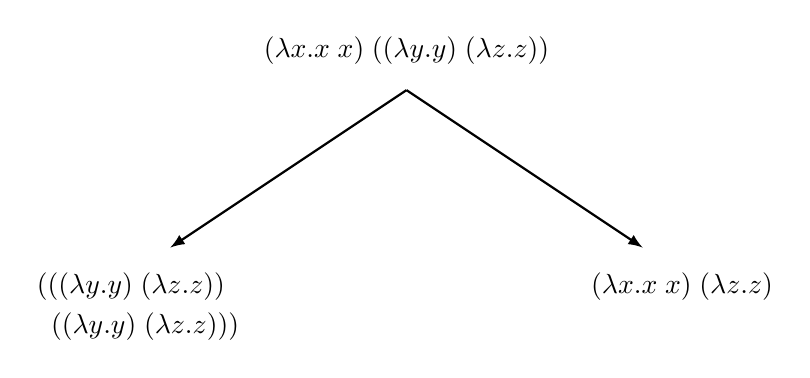
\begin{tikzpicture}
\begin{scope}[thick,>=latex]
\draw [->] (3,2) -- (0,0);
\draw [->] (3,2) -- (6,0);
\node at (3,2.5) {$(\lambda{}x.x\;x)\;((\lambda{}y.y)\;(\lambda{}z.z))$};
\node at (-0.5,-0.5) {$(((\lambda{}y.y)\;(\lambda{}z.z))$};
\node at (-0.32,-1) {$((\lambda{}y.y)\;(\lambda{}z.z)))$};
\node at (6.5,-0.5) {$(\lambda{}x.x\;x)\;(\lambda{}z.z)$};
\end{scope}
\end{tikzpicture}
\end{center}

\indent{}需要注意的是,有些$\lambda$-演算表达式是没有标准型的。例如,下面的表达式$\Omega$就没有标准型:
\begin{displaymath}
\Omega \doteq ((\lambda{}x.x\;x)\;(\lambda{}x.x\;x))
\end{displaymath}
\noindent{}即使一个表达式有标准型,在归约的时候也可能会产生无限的归约序列。例如:
\begin{align*}
&(\lambda{}y.\lambda{}z\;z)\;((\lambda{}x.x\;x)\;(\lambda{}w.w\;w))\\
&\begin{array}{lll}
\rightarrow_{\bf{n}} & \lambda{}z.z & \textrm{\small\color{gray}{标准型}}\\
\\
\rightarrow_{\bf{n}} & (\lambda{}y.\lambda{}z\;z)\;((\lambda{}w.w\;w)\;(\lambda{}w.w\;w)) &\\
\rightarrow_{\bf{n}} & (\lambda{}y.\lambda{}z\;z)\;((\lambda{}w.w\;w)\;(\lambda{}w.w\;w)) &\\
\rightarrow_{\bf{n}} & \cdots & \textrm{\small\color{gray}{永远重复相同的表达式}}
\end{array}
\end{align*}

\indent{}尽管定理\;\ref{theorem:NF}\;说明最多存在一个标准型,但目前我们还没有得到寻找它的确切方式。直觉上,之所以
会出现上面这种无法停止的归约序列,是因为我们在对函数体中未被用到的参数求值。这表明了一种策略,即应用表达式中最左侧
的$\beta$或$\eta$归约:
\begin{tcolorbox}[top=-0.4em,left=0mm,right=0mm]
\begin{gather*}
\begin{array}{lll}
M \rightarrow_{\bar{\bf{n}}} N & \textrm{if} & M\;\beta\;N\\
M \rightarrow_{\bar{\bf{n}}} N & \textrm{if} & M\;\eta\;N\\
(M\;N) \rightarrow_{\bar{\bf{n}}} (M'\;N) & \textrm{if} & M \rightarrow_{\bar{\bf{n}}} M'\\
& \textrm{and} & \forall{}L,(M\;N)\not\!\beta\;L\textrm{ and }(M\;N)\not\!\eta\;L\\
(M\;N) \rightarrow_{\bar{\bf{n}}} (M\;N') & \textrm{if} & N \rightarrow_{\bar{\bf{n}}} N'\\
& \textrm{and} & M\textrm{ is in normal form}\\
& \textrm{and} & \forall{}L,(M\;N)\not\!\beta\;L\textrm{ and }(M\;N)\not\!\eta\;L
\end{array}
\end{gather*}
\end{tcolorbox}
\noindent{}式中的$\rightarrow_{\bar{\bf{n}}}$关系是\textbf{normal-order reduction}关系。若存在标准型,则保证能找到它。

\begin{theorem}
\textbf{Normal Order Reduction - }$M$有标准型$N$当且仅当$M\twoheadrightarrow_{\bar{\bf{n}}}N$。
\end{theorem}

\indent{}Normal Order Reduction也叫\textbf{call-by-name}。尽管它能在标准型存在时找到标准型,但是在实践上并没有
编程语言使用这种形式的归约,原因是它很慢(虽然功能确实很强)。

\end{document}